%second chapter of your thesis
\chapter{Literatuurstudie}

In dit hoofdstuk zal er eerst een korte overzicht voorzien worden van het kader waarin de thesis zich voordoet. Hierna zal een kleine inleiding gegeven worden tot Artifici\"ele Intelligentie: welke verschillende vormen bestaan er en wat zijn de mogelijke toepassingsdomeinen. De verschillende leermodellen worden bekeken en wordt er nagegaan hoe de onderdelen een werkend geheel vormen.  Vervolgens wordt er een overzicht van de voor- en nadelen van de verschillende technieken. Er wordt een best bruikbare methode voor de toepassing in deze thesis gekozen. Bij deze keuze zullen de voor- en nadelen gewikt en gewogen worden. Verder wordt er ook de geschiedenis van Single Board Computers aangehaald. Hoe zijn deze toestellen ontstaan, hoe zijn ze ge\"evolueerd en in welke staat zijn de hedendaagse SBCs. Verder worden ook verschillende voorbeelden van SBCs besproken die in staat zijn om Machine Learning-technieken toe te passen. Deze zullen onderworpen worden aan een benchmark die we in paragraaf ~\ref{benchmark} bespreken.

\newpage

\section{Kadering masterproef}

De computerwereld maakt de laatste jaren grote stappen op vlak van Machine Learning\cite{Minar18}. Deze vorderingen werden gedreven door onder meer de nieuwste ontwikkelingen op vlak van computerrekenkracht en de vierde industri\"ele revolutie\cite{bloem2014fourth}. Door de veelvuldige toepassingsmogelijkheden werd \gls{ml} een populair en veelbesproken onderwerp. Tegenwoordig kan een bepaalde vorm van \gls{ai} in elke sector teruggevonden worden. Van hartritmestoornissen in de medische sector tot commentaarherkenning in de toeristische stiel. 

Een branche in de \gls{ml} die steeds meer in de schijnwerpers staat, is in de logistieke sector\cite{barreto2017industry}. Door de steeds verder doorgedreven automatisatie van bedrijven, wordt er ook in bijvoorbeeld magazijnen geopteerd voor het optimaliseren van onder meer het leveren van de verschillende onderdelen en de veiligheid in het magazijn.. Gebruik maken van zelfrijdende vorkheftrucks is een mogelijke optie in het verbeteren van de effici\"entie. Niet alleen in het magazijn maar ook op de weg is er een groeiende belangstelling naar zelfrijdende auto's, die ontwikkeld worden door grote bedrijven zoals Tesla en Uber. In beide cases zal er een zekere vorm van positiebepaling nodig zijn. Het is van groot belang dat deze bepaling zo accuraat mogelijk plaats vindt, met niet alleen een juiste locatie, maar ook op zo kort mogelijke tijdsperiode. Deze nood aan \textit{low latency} kan het verschil betekenen tussen een voertuig die beslist dat hij moet vertragen of beslist dat hij veilig kan doorrijden maar toch een botsing veroorzaakt. De berekening van de locatiebepaling kan zowel in de \textit{cloud}, als in de \textit{edge}\cite{edgecomputingLi} gebeuren en gebeurt vooral met behulp van \gls{ml}. Door een toegevoegde latency van meerdere tientallen milliseconden bij berekeningen in de cloud zal de keuze voor \textit{edge computing} vallen. Welke hardware men gebruikt kan vari\"eren van applicatie tot applicatie.

In deze thesis zal men trachten de edge-kant te belichten door een benchmark op te stellen. Dit instrument moet meer inzicht verschaffen in welke mate machineleertechnieken toepasbaar zijn. Hoe groot is de latency die op treed? Welk verbruik en complexiteit van het netwerk gaat er hier mee gepaard? De benchmark zal toegepast worden op verschillende Single Board Computers. Ook tussen deze hardware-opties wordt er een afweging gemaakt. Welk toestel is voordeliger in welke situatie? Is een goedkoper toestel tot evenwaardige resultaten in staat?



\newpage

\section{\gls{ml}}
\gls{ml} is een onderdeel van \gls{ai} en staat voor het wetenschappelijke onderzoek naar algoritmes en statistische modellen dat gebruikt kan worden door verschillende computersystemen. Deze systemen zijn hierdoor in staat om specifieke taken te voltooien zonder rechtstreekse instructies of regels mee gekregen te hebben. Ze steunen onder meer op patroonherkenning om de kans op het succesvol uit voeren van taken te maximaliseren. Hiervoor wordt er een wiskundig model gebouwd op basis van training-data. Dit mathematisch modelleren en \textit{datahandling} kunnen op verscheidene manieren gebeuren. Hieronder bespreken we een aantal gebruikelijke modellen. We maken ook een afweging welk model het meest interessant is voor onze toepassing. 

\subsection{Leermodellen}
Om \gls{ml} technieken toe te passen moet men gebruik maken van een bepaald model. Een model dat is toegepast op trainingsdata en nieuwe data kan verwerken om voorspellingen te maken. Er bestaat een hele waaier aan mogelijke modellen. In de volgende paragrafen bespreken we een aantal opties waarna we de verschillende modellen afwegen tegenover elkaar.

	\subsubsection{Artifici\"ele Neurale Netwerken}
	\gls{ann} is een term die gebruikt wordt om een algoritme te omschrijven dat lijkt op, maar niet hetzelfde is als een biologisch neuraal netwerk in de hersenen van dieren. Deze systemen zijn in staat om een bepaalde taak te leren, en zichzelf te verbeteren. In de meeste gevallen worden er zelfs geen richtlijnen of een omschrijving meegegeven. Het systeem ontdekt zelf hoe deze regels in elkaar zitten. Een bekend voorbeeld is het herkennen van de cijfers 0 tot 9. Hierin wordt er niet aan het systeem verteld dat het cijfer 8 uit twee cirkels bestaat die verticaal tegen elkaar aansluiten. Het algoritme zal dit gaandeweg ontdekken met behulp van de vele voorbeelden waar het gebruik van kan maken. Met behulp van veel data kan een algoritme zichzelf verfijnen en nauwkeuriger bepaalde cijfers herkennen.
	
		\paragraph{Structuur van \gls{nn}}
		Een \gls{ann} is een verzameling van nodes die met elkaar verbonden zijn zoals neuronen in de hersenen van een mens. Hierbij kan elke neuron een signaal doorgeven naar het volgend neuron waar het signaal verwerkt kan worden en weer doorgegeven kan worden. Hetzelfde principe geldt ook bij \gls{nn} met het verschil dat er meerdere lagen van nodes te onderscheiden zijn. 
	
		\begin{figure}
			\centering
			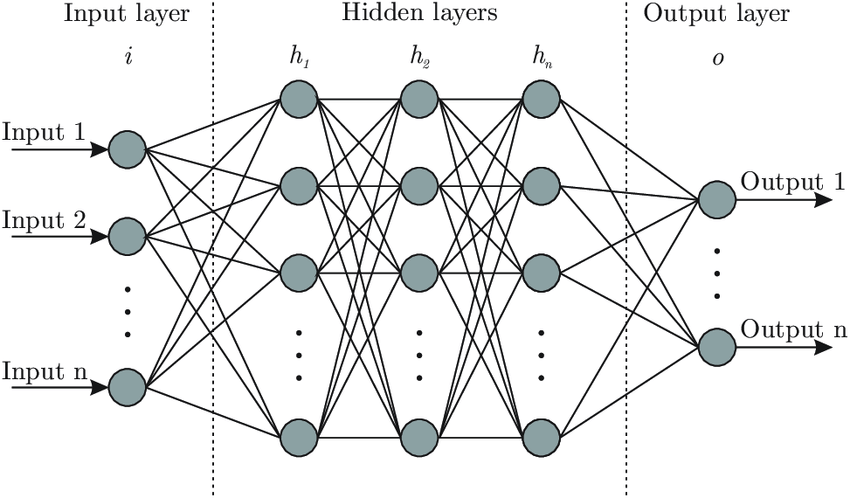
\includegraphics[width=140mm]{afbeeldingen/neuralNetwork2.PNG}
			\caption{Structuur van een Neuraal Netwerk}
			\label{fig:neuralNetworkStructuur}
		\end{figure}
		
			\subparagraph{Lagen}
			Er zijn drie soorten lagen te onderscheiden: een Input Layer, Hidden Layers en een Output Layer. Elke laag is verbonden met de volgende laag door middel van connecties of \textit{edges} tussen de verschillende nodes. In figuur ~\ref{fig:neuralNetworkStructuur} is de algemene vorm te vinden van een \gls{nn}.
		
				\begin{itemize}
					\item \textbf{Input Layer:} De eerste laag van elk \gls{nn} is de Input Layer. Deze bestaat uit een aantal inputnodes. Elke inputnode krijgt de ruwe data binnen waar er een operatie op uitgevoerd wordt en vervolgens bepaalde parameters doorgeeft aan de volgende laag. 
					\item \textbf{Hidden Layers:}  Na de inputlaag komen een aantal Hidden Layers. Het aantal Hidden Layers en de hoeveelheid nodes binnen \'e\'en Hidden Layer kan vari\"eren van applicatie tot applicatie en is sterk gerelateerd aan de complexiteit van de toepassing.
					\item \textbf{Output Layer:} Na de Hidden Layers is de laatste laag de Output Layer. Hier worden de laatste operaties uitgevoerd en worden de eindwaarden verkregen.
				\end{itemize}
			
			\subparagraph{Nodes}
			Een node is gebaseerd op zijn biologisch tegenbeeld. Het krijgt een bepaald aantal inputs, verwerkt deze en geeft een bepaald aantal outputs. Deze inputs en outputs worden van node naar node doorgegeven via verbindingen. Elke node heeft met elke node in de volgende laag een connectie. Deze worden \textit{edges} genoemd. Elke edge draagt een bepaald gewicht. Via dit gewicht kan men de invloed van de  huidige node versterken of verzwakken in de volgende node.
	
			\subparagraph{Propagation function}
			De mathematische functie die een node gebruikt voor het verwerken van inputs naar outputs heet de propagatie functie.
			In figuur ~\ref{fig:artificial_neuron} bespreken we de algemene vorm van een neuron voor een bepaalde neuron met m+1 inputs $\left(  x_0 t.e.m. x_m \right) $ en bijhorende gewichten $\left(  w_0 t.e.m. w_m \right) $.
			Gebruikelijk wordt $x_0 = +1$ genomen. Hierdoor blijven er maar m echte inputs over waardoor er voor een bepaalde output volgende functie opgesteld kan worden. Hierbij is $\phi$ een van de mogelijke transferfuncties die verder besproken zal worden.

			\begin{equation}
				y_k = \phi \left( \sum_{j=0}^{m}w_{kj}x_j\right) 
			\end{equation}
			
			\begin{figure}
				\centering
				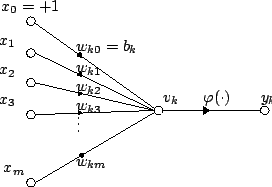
\includegraphics[width=60mm]{afbeeldingen/Artificial_neuron.PNG}
				\caption{Algemene structuur van een node.}
				\label{fig:artificial_neuron}
			\end{figure}
			
			\subparagraph{types transferfuncties}
			De transfer functie of activatiefunctie van een neuron bevat bepaalde eigenschappen die het volledige netwerk kan verbeteren of vereenvoudigen. Hieronder bespreken we enkele transferfuncties.
			
			\begin{itemize}
				\item \textbf{Stapfunctie:} Hier wordt er gekeken naar de verkregen waarde van de gewogen som u van m+1 inputs. Bedraagt deze waarde minder dan een bepaalde drempel $\theta$, dan wordt de output gelijkgesteld aan nul, bij een hogere waarde dan weer aan 1. Dit is te zien in formule ~\ref{eq:stapfunctie}. Dit type wordt vooral gebruikt om binaire inputs te verzorgen bij de volgende laag. 
				\begin{equation}
				u =  \left( \sum_{j=0}^{m}w_{kj}x_j\right) 
				\end{equation}
				\begin{equation}\label{eq:stapfunctie}
				y={\begin{cases}1&{\text{als }}u\geq \theta
					\\0&{\text{als }}u<\theta \end{cases}}
				\end{equation}
				
				\item \textbf{Lineare Combinaties:} In dit geval is de output niets minder dan de gewogen som vermenigvuldigd met een constante waarbij een tweede constante wordt opgeteld.
				\item \textbf{Sigmoid:} De Sigmoid functie is een mathematische functie die lineaire inputs omzet naar niet-lineaire outputs. Het heeft de karakteristieke 'S'-vorm zoals te zien is in ~\ref{fig:sigmoid}. Door deze activatiefunctie worden inputs omgezet in een waarde tussen 0 en 1 (of -1 en 1, afhankelijk van de conventie).
				\item \textbf{Rectifier:} De rectifier als activatiefunctie is een functie die enkel het positieve deel van zijn argument doorlaat. In vergelijking ~\ref{eq:rectifier} vind je de functie weer waar x de input is van de neuron. Deze is een vector aan waarden die zowel positief als negatief kunnen zijn. Deze functie is ook gekend onder de naam \textit{\gls{relu}}.
				\begin{equation}\label{eq:rectifier}
				f(x) = x^+ = max(0,x)
				\end{equation}
			\end{itemize}
			
			\begin{figure}
				\centering
				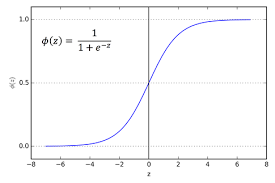
\includegraphics[width=70mm]{afbeeldingen/sigmoid.PNG}
				\caption{De Sigmoid activatiefunctie\citep{bron:sigmoidfoto}.}
				\label{fig:sigmoid}
			\end{figure}
	\subsubsection{Beslissingsboom} 
	Het gebruik van een beslissingsboom is een leermethode die met regelmaat terugkomt in de statistiek als een voorspellend model. Men maakt gebruik van observaties rond een bepaald onderwerp om een beslissing te nemen rond de aard van het onderwerp. Deze beslissing leidt naar een variabele outputwaarde. Indien deze waarde valt onder te verdelen in discrete klassen spreekt men over een \textit{classificatie boom}. Neemt de gezochte variabele eerder een continue vorm aan, dan maakt men gebruik van \textit{regressie bomen}.
	

	
		\paragraph{Structuur van een beslissingsboom}
		
		
		Net zoals bij de \gls{nn} bestaat een beslissingsboom uit verschillende lagen en nodes. Er zijn echter wel belangrijke verschillen in het gebruik bij \gls{nn} en een beslissingsboom. Eerst en vooral worden lagen horizontaal weergegeven t.o.v. verticaal bij Neurale Netwerken. Zoals te zien is in figuur ~\ref{fig:beslissingsBoom} wordt er in elke laag een onderscheid gemaakt op basis van een bepaalde statement of parameter. Deze parameter kan een enkele inputwaarde zijn of een lineaire combinatie van meerdere inputwaarden. 
		
		Bij de nodes kan er onderscheid gemaakt worden tussen een gewone node en een eindnode. Bij elke gewone node wordt een bepaalde statement geverifi\"eerd en wordt er naar een node overgegaan in de volgende laag op basis van dit statement. Bij een eindnode is het niet meer mogelijk om door te gaan naar een volgende laag, maar wordt er een outputwaarde gegeven.
		
		\begin{figure}
			\centering
			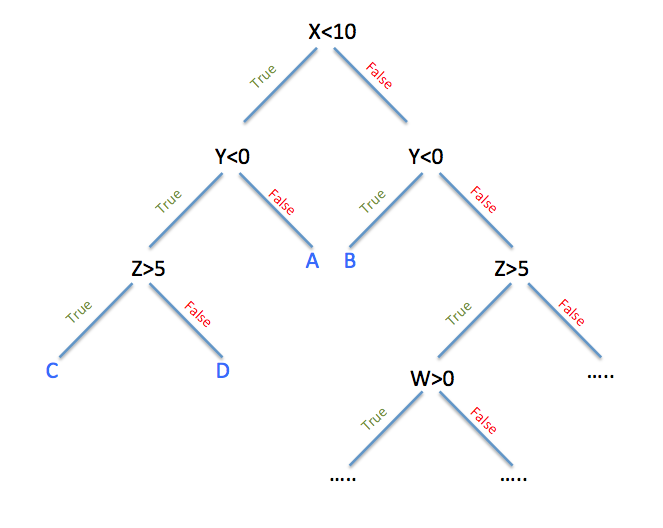
\includegraphics[width=80mm]{afbeeldingen/beslissingsBoom.PNG}
			\caption{Algemene structuur van een beslissingsboom.\citep{bron:beslissingsboom}}
			\label{fig:beslissingsBoom}
			%bron: https://medium.com/machine-learning-bites/machine-learning-decision-tree-classifier-9eb67cad263e
		\end{figure}
		
		
	
	
	\subsubsection{Support Vector Machines}
	\gls{svm} of ook wel gekend als support vector networks is een model dat veelvuldig gebruikt wordt in classificatie en regressie-analyse. \gls{svm} verdeelt objecten onder in twee verschillende klassen aan de hand van een aantal kenmerken. Het is dus een binaire classificeerder. Om aan de hand van kenmerken een onderverdeling te maken moeten deze kenmerken eerst omgezet worden in een numeriek model. De data worden hervormd tot een vectorruimte. In de trainingsfase wordt er getracht een zo optimaal mogelijke scheiding tussen beide klassen te vinden. Deze optimale scheiding wordt ook wel een \textit{hypervlak} genoemd en ligt op een zo groot mogelijke afstand tussen de dichtstbijgelegen objecten van beide klasses of support vectors. in figuur ~\ref{fig:supportVectorMachines} kan u een twee dimensionaal voorbeeld vinden. Hierin is scheidingslijn H1 geen acceptabele scheiding omdat er objecten van de zwarte klasse fout geclassificeerd worden. H2 is acceptabel maar is nog niet optimaal aangezien er weinig foutmarge is voor een nieuw object. H3 is het hypervlak omdat de foutenmarge tussen de twee klassen zo groot mogelijk is. Deze methode is niet alleen bruikbaar in toepassingen met een lineaire scheiding. Ook in niet-lineaire gevallen kan men een transformatie uitvoeren om toch een lineaire scheiding te bekomen. Deze hervorming wordt ook wel de \textit{kernel trick} genoemd. 
	
	
	\begin{figure}
		\centering
		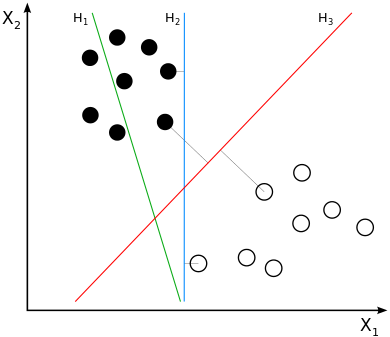
\includegraphics[width=80mm]{afbeeldingen/supportVectorMachines.PNG}
		\caption{Twee dimensionale Support Vector Machine.\citep{bron:supportvectormachines}}
		\label{fig:supportVectorMachines}
		%bron: https://subscription.packtpub.com/book/big_data_and_business_intelligence/9781788994170/5/ch05lvl1sec36/support-vector-machines
	\end{figure}
		
			
	\subsubsection{Regressie Analyse}
	Regressie Analyse is techniek uit de statistiek, die gebruikt wordt om gegevens te analyseren met een specifiek verband. Er bestaat vaak een relatie tussen een afhankelijke variabele en \'e\'en (of meerdere) onafhankelijke variabelen. De meest voorkomende vorm van regressie analyse is de lineaire regressie, waar men op zoek gaat naar de functie die het dichtst aanleunt bij de data en dit volgens specifieke criteria, zoals het voldoen aan een bepaalde graad. Regressie analyse wordt vooral gebruikt voor het voorspellen van nieuwe data of gebeurtenissen. In figuur ~\ref{fig:regressieAnalyse} kan je een voorbeeld van lineaire regressie vinden.
	\begin{figure}
		\centering
		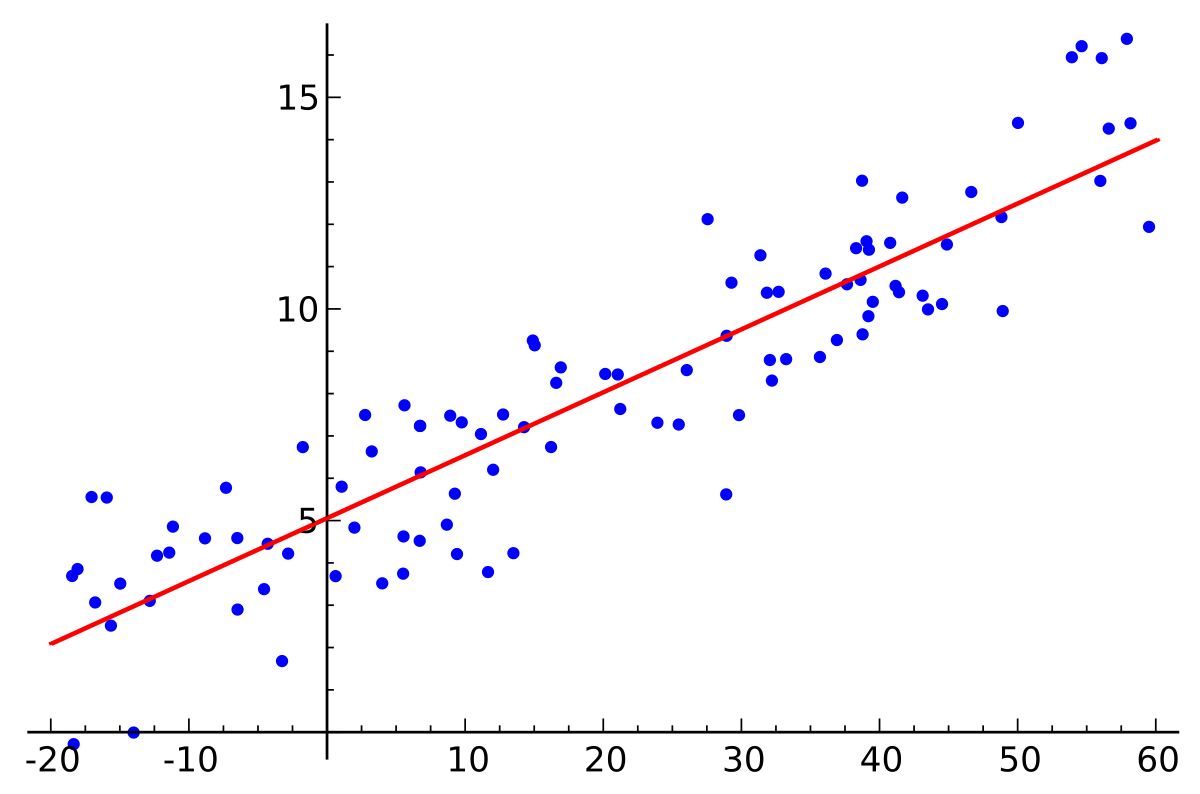
\includegraphics[width=80mm]{afbeeldingen/regressieAnalyse.PNG}
		\caption{Voorbeeld van Lineaire Regressie.\citep{bron:regressieanalyse} }
		\label{fig:regressieAnalyse}
		
		%bron: https://en.wikipedia.org/wiki/Regression_analysis
	\end{figure}
	
	
	\subsubsection{Bayesian Netwerken}
	Bayesian Netwerken, ook wel probabilistische netwerken genoemd, zijn structuren waarin data op probabilistische wijze geanalyseerd kan worden. Men maakt gebruik van gerichte grafen. Hierin bestaan de knopen uit variabelen en de arcs beschrijven de conditionele afhankelijkheden tussen de verschillende knopen. Bayesian Netwerken worden vooral gebruikt om te analyseren wat de bepalende oorzaak is voor een zekere gebeurtenis. 
	
	\subsubsection{Genetisch Algoritmes}
	Genetische Algoritmes zijn een heuristiek ge\"inspireerd op het principe van natuurlijke selectie en zijn een klasse binnen evolutionaire algoritmes. Dit type algoritme kan gebruikt worden om oplossingen te vinden in optimalisatie- en zoekproblemen. Door te steunen op biologische principes zoals mutatie, selectie en kruisbestuiving worden er nieuwe \textit{chromosomen} gegenereerd die mogelijks een betere oplossing geven voor een bepaald probleem.
	
\subsection{Keuze voor een \gls{ml}-methode }	
% https://elitedatascience.com/machine-learning-algorithms

Om de keuze voor een bepaalde \gls{ml}-techniek te verantwoorden bespreken we in dit hoofdstuk de voor- en nadelen van de voornaamste technieken die via regressie en classificatie toegepast kunnen worden.\cite{bron:mlalgoritmes}

	\subsubsection{Regressie}

	\begin{itemize}
		\item \textbf{Neurale Netwerken:}
			\subitem Voordelen: Neurale netwerken zijn de huidige state-of-the-art in verschillende domeinen. \gls{nn} kunnen uitstekend omgaan met onder meer beeld-, audio- en tekstdata en deze verwerken. Verder kan de architectuur ook nog gemakkelijk aangepast worden aan de toepassing door te vari\"eren in het aantal lagen of nodes. Het gebruik van de hidden layers vermindert ook het hanteren van feature engineering. 
			\subitem Nadelen: Neurale netwerken zijn minder bruikbaar voor \textit{general-purpose} algoritmes door de grote hoeveelheid data die er voor nodig zijn. In dat geval is het beter om voor beslissingsbomen te kiezen. Bovendien vragen ze veel vermogen voor het trainen van het netwerk en vragen veel expertise voor kleine aanpassingen zoals architectuur en hyperparameters. 
		\item \textbf{Regression Trees:}
			\subitem Voordelen: Beslissingsbomen met nadruk op regressie zijn in staat om niet-lineaire relaties te leren en zijn robuust voor uitschieters in de te verwerken dataset.
			\subitem Nadelen: Regression trees zijn vatbaar voor overfitting indien er te veel gebruik gemaakt wordt van branches. Bomen hebben vaak de neiging om branches aan te maken tot het een exacte kopie voorstelt van de trainingsdata.
		\item \textbf{Lineaire Regressie:}
			\subitem Voordelen: Dit is een eenvoudige methode om zowel te verstaan als uit te leggen. Daarnaast kan er bescherming tegen overfitting ge\"implementeerd worden. 
			\subitem Nadelen: Niet-lineaire relaties zijn een zwak punt voor lineaire regressie. Het is moeilijk om een correcte fitting te vinden voor een gegeven netelige relatie. Bovendien is het onvoldoende flexibel om complexe patronen op te vangen.

	\end{itemize}

	\subsubsection{Classificatie}
	
	\begin{itemize}
		\item \textbf{Neurale Netwerken:}
			\subitem Voordelen: Neurale werken blijven uitstekend presteren bij het classificeren van audio-, tekst- en beeldherkenning.
			\subitem Nadelen: Er is nood aan grote hoeveelheden data om het model te trainen en minder geschikt als general-purpose algoritmes.
		\item \textbf{Classification Trees:}
			\subitem Voordelen: Verrichten zeer goed werk in praktijk. Ze zijn robuust voor uitschieters, schaalbaar voor meerdere klassen en kunnen niet-lineaire grenzen op natuurlijke wijze modelleren dankzij de hi\"erarchische structuur.
			\subitem Nadelen: Classification trees zijn vatbaar voor overfitting indien er te veel gebruik gemaakt wordt van branches. Bomen hebben vaak de neiging om branches aan te maken tot het een exacte kopie voorstelt van de trainingsdata.
		\item \textbf{Support Vector Machines:}
			\subitem Voordelen: \gls{svm} zijn in staat om niet-lineaire beslissingsgrenzen te modelleren en hebben een sterke robuustheid tegen overfitting, vooral in hogere dimensionale vectorruimtes.
			\subitem Nadelen: \gls{svm} zijn heel erg geheugen intensief. Ze vragen ook meer expertise in het afstemmen door het grote aanbod in mogelijke kernels. \gls{svm} hebben de eigenschap om minder effectief te zijn bij het schalen naar grotere datasets. 
		\item \textbf{Geregulariseerde Regressie:}		
			\subitem Voordelen: Outputs hebben een  gemakkelijk leesbare probabilistische interpretatie. Ook kan er bescherming tegen overfitting ge\"implementeerd worden en kunnen modellen eenvoudig ge\"updatet worden.
			\subitem Nadelen: Niet-lineaire relaties zijn een zwak punt voor lineaire regressie. Het is moeilijk om een correcte fitting te vinden voor een gegeven netelige relatie. Bovendien is het onvoldoende flexibel om complexe patronen op te vangen.

			
	\end{itemize}

	\subsubsection{Besluit}
	Na een afweging gedaan te hebben van de belangrijkste kandidaten bij zowel regressie als classificatie toepassingen kunnen we besluiten dat Neurale Netwerken een goede keuze is als model. We steunen vooral op het feit dat \gls{nn} uitstekend werk levert in beide klassen in het analyseren van data. Bovendien zijn de voornaamste nadelen minder van toepassing in het kader waarin \gls{nn} toegepast zal worden. Het is vooral van belang hoe de netwerken in de executiefase presteren. Het trainen van de verschillende netwerken met grote hoeveelheden data kan op aparte systemen gebeuren. De trainingsfase is dus minder van belang voor het doel van deze thesis. Bovendien is het niet nodig om een breed general-purpose netwerk te voorzien.
	
	Een mogelijk alternatief voor \gls{nn} is het gebruiken van Regressie Analyse. De bepalende factor hiervoor is dat het karakter van de verscheidene applicaties vaak uit lineaire relaties bestaat. 
		
		
		
		
\newpage
\subsection{Leertechnieken}
er zijn verschillende mogelijkheden van een neuraal netwerk te laten leren. De drie belangrijkste methodes om een mathematische functie te verkrijgen worden hieronder opgesomd.


	\subsubsection{Supervised Learning} Deze techniek maakt gebruik van gepaarde datasets van inputobjecten en de te verwachten outputobjecten. Het doel is om een mathematische functie te cre\"eren waarbij de gegenereerde outputs zo nauw mogelijk overeenkomen met de gelabelde outputs uit de datasets. Men optimaliseert deze mathematische functie door iteratief te trainen. De bijgeschaafde functie kan dan ook gebruikt worden voor nieuwe datasets zonder gelabelde output. Een toepassing van Supervised Learning is bijvoorbeeld het detecteren van spam met een trainingset van al gelabelde e-mails.
	
	\subsubsection{Unsupervised Learning} Unsupervised learning is een techniek dat gebruik maakt van Hebbian Learning om onbekende patronen te herkennen in datasets. De twee meest gebruikte methodes onder Unsupervised Learning zijn principal component en cluster analysis. Principal component maakt gebruik van orthogonale transformaties om een set van mogelijke afhankelijke variabelen om te zetten in een set van lineaire onafhankelijke variabelen. In cluster analyse wordt er getracht om een groep objecten te identificeren en te verdelen in een cluster van gelijkaardige objecten. 
	Een belangrijke toepassing van Unsupervised Learning is het clusteren van gelijkaardige documenten op basis van de inhoud van de tekst.
	
	% Discovering patterns in unlabeled data Example: cluster similar documents based on the text content
	
	\subsubsection{Reinforcement Learning} Deze leertechniek heeft betrekking tot hoe agents acties moeten ondernemen in een omgeving om een bepaald attribuut te maximaliseren. Het onderscheidt zich van Supervised en Unsupervised Learning door de onafhankelijkheid van gelabelde outputdatasets. Hierbij worden bovendien minder optimale acties niet manueel gecorrigeerd. De techniek heeft als doel om een evenwicht te vinden tussen exploratie van ongekend gebied en exploitatie van de huidige kennis. In figuur ~\ref{fig:reinforcemntLearning} kan je een eenvoudige routine vinden van Reinforcement Learning-algoritme. Hierbij maakt een agent een bepaalde actie gebaseerd op de staat waar hij in is. Deze actie heeft in een omgeving een zekere invloed die door een Interpreter beoordeeld wordt en een score toekent. De agent kan deze verandering daarna gebruiken om zichzelf te verbeteren en zijn acties aanpassen. 
	\begin{figure}
		\centering
		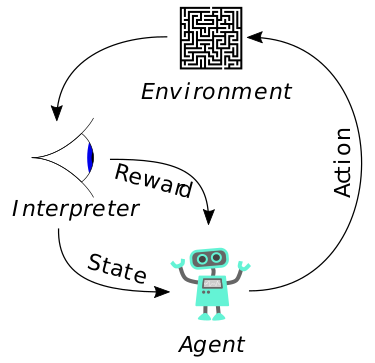
\includegraphics[width=60mm]{afbeeldingen/Reinforcement_learning_diagram.PNG}
		\caption{Routine bij Reinforcement Learning}
		\label{fig:reinforcemntLearning}
	\end{figure}
	Een van de vele mogelijke toepassingen van Reinforcement Learning is het aanleren van schaken door enkel mee te geven of het algoritme gewonnen of verloren heeft. 
	

\newpage	

%------------------------------------------------------------------------------	
\section{Evolutie \gls{sbc}}
Een \gls{sbc} is een volledige computer gemaakt op 1 enkele printplaat. Het bevat onderdelen zoals een microprocessor, geheugen, inputs en outputs. De \gls{sbc} werd ontwikkeld als een voorstel-hulpmiddel bij educatieve doelstellingen of het gebruik als een embedded computer controller. Tegenwoordig zijn ook vele (draagbare) computers ge\"integreerd op \'e\'en printplaat. Het grote verschil met (draagbare) computers is dat er geen nood is aan expansion slots zoals bijvoorbeeld voor RAM-geheugen of een \gls{gpu}.
	\subsection{Geschiedenis}
	De eerste echte SBC was de zogenaamde "dyna-micro"\space uit figuur ~\ref{fig:eersteSBC} die later de naam "MMD-1" (Mini-Micro Designer 1) kreeg. Dit toestel werd uitgegeven in 1976 en werd populair doordat het werd gepresenteerd in het destijds 'BugBook' als het voorbeeld microprocessor. Een andere vroege \gls{sbc} was de KIM-1 (Keyboard Input Monitor 1) uit hetzelfde jaar. Beide machines werden voor ingenieurs geproduceerd en ontworpen maar vonden een breed publiek onder de hobbyisten waar het heel populair was. Later kwamen nog andere namen zoals de Ferguson Big Board en de Nascom.

	\begin{figure}
		\centering
		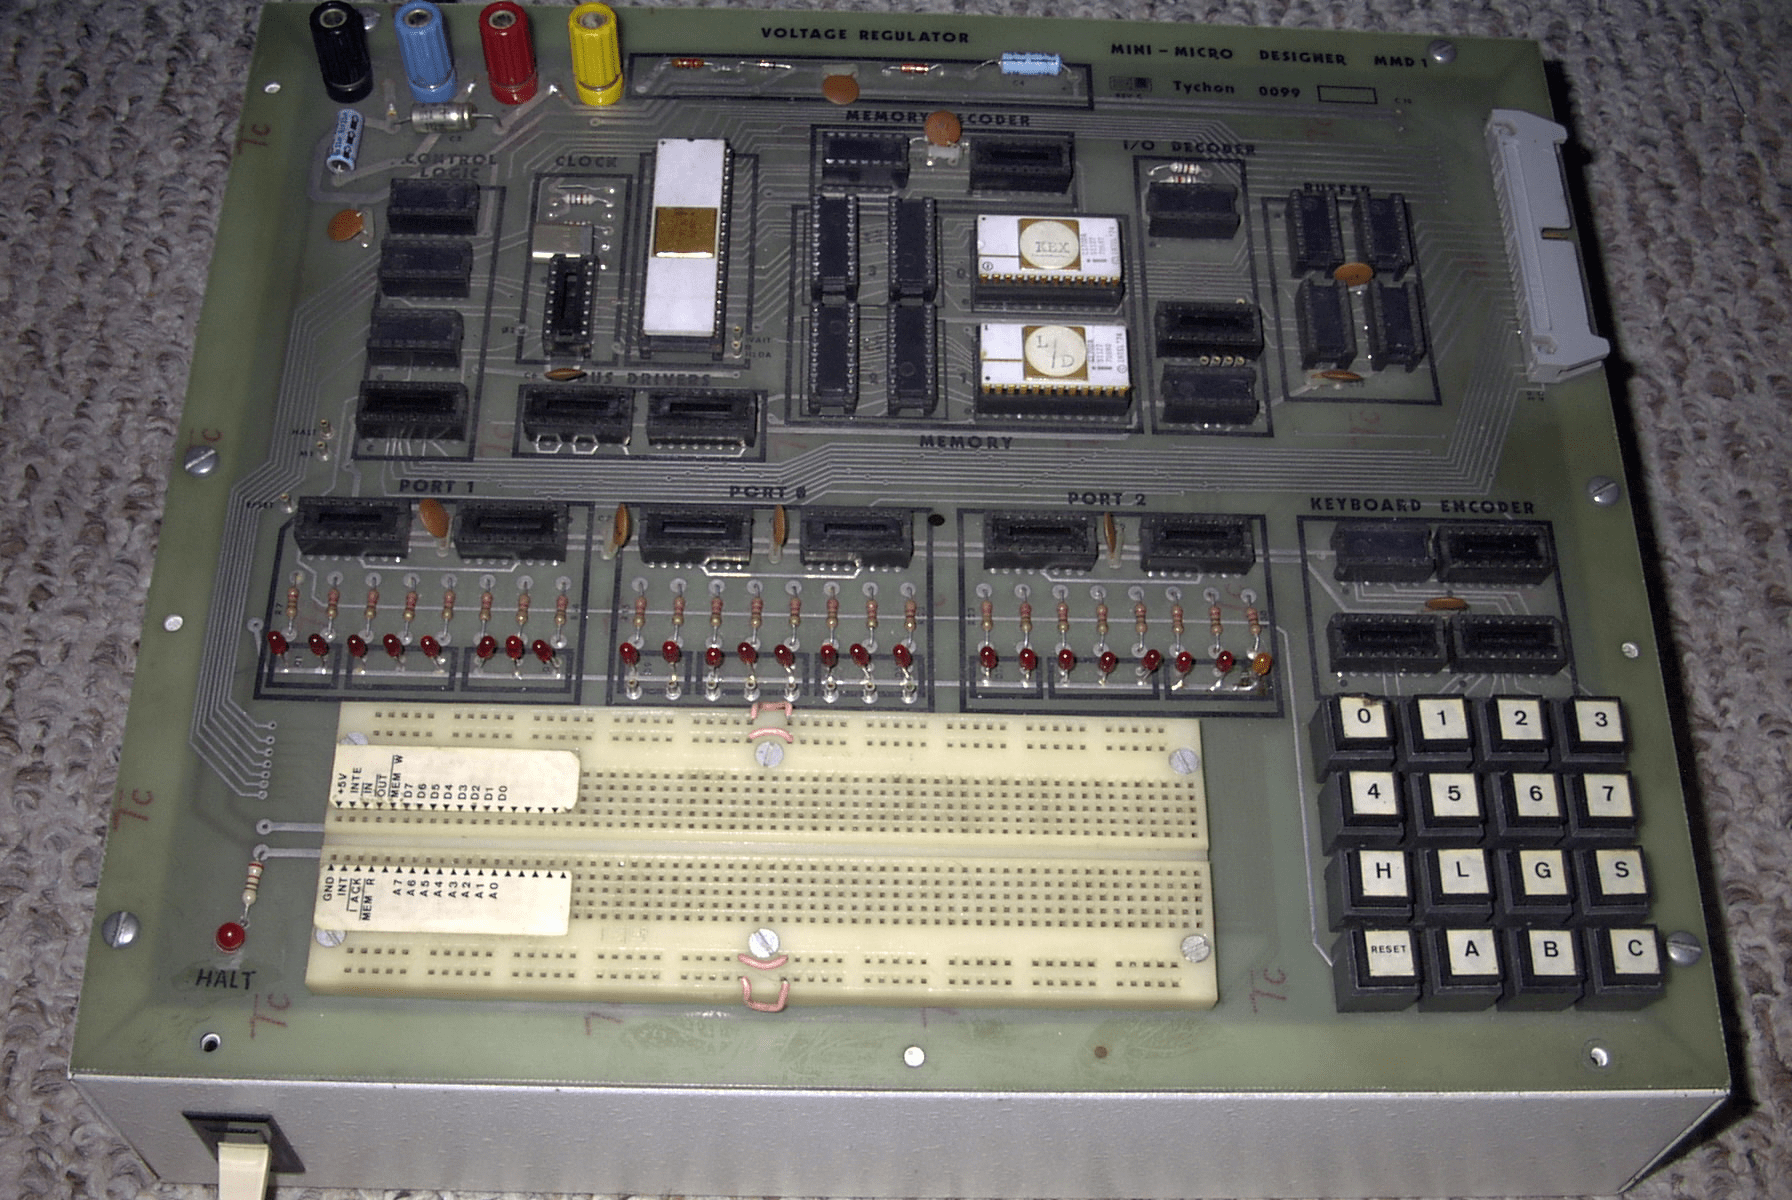
\includegraphics[width=120mm]{afbeeldingen/Early_1976_MMD1_Prototype_most_chips_removed.PNG}
		\caption{Eerste \gls{sbc}: MMD-1 \cite{bron:fotoeerstesbc}}
		\label{fig:eersteSBC}
	\end{figure}
	
	Naarmate de markt voor desktops en PC's groeide, nam de belangstelling voor \gls{sbc} in computers meer en meer af. De focus van de markt werd verlegd naar een moederbord met de belangrijkste componenten en dochterborden voor periferiecomponenten zoals seriële poorten. De voornaamste reden hiervoor was dat de componenten groot waren. Alle onderdelen op dezelfde printplaat zou zorgen voor een onpraktisch ontwerp met grote afmetingen. Deze beweging was echter tijdelijk en naarmate de vorderende technologie kleinere componenten kon leveren, werden onderdelen terug naar het mainframe verschoven. Tegenwoordig kunnen de meeste moederborden terug als \gls{sbc} beschouwd worden. 

	
	In het jaar 2004 werd er in Itali\"e een nieuwe microcontroller uitgebracht onder de naam "Arduino". Dit ontwerp had, naast het voordeel van compact en goedkoop te zijn, ook nog eenvoudigheid mee. Door de eenvoud werd het Arduino-platform snel populair onder techneuten van alle soorten. 
	Twee jaar later bracht de Universiteit van Cambridge een nieuwe goedkope \gls{sbc} uit. De bekende Raspberry Pi werd gelanceerd voor de prijs van \$35. Het hoofddoel van dit project was een nieuw leermiddel om te programmeren maar werd door het grote aantal applicaties ook zeer populair. \label{raspberry}
	
	De laatste jaren kende een grote explosie aan nieuwe \gls{sbc}s. Een hele reeks nieuwe namen verscheen. Banana Pi, Beaglebone, Intel Galileo, Google Coral Dev en Asus Tinker Board zijn maar enkele van de vele voorbeelden. Deze toestellen hebben vaak een processor gebaseerd op de x86- of ARM-series en maken gebruik van een Linux besturingssysteem zoals Debian.
	

% https://nl.wikipedia.org/wiki/Singleboardcomputer

\newpage


%------------------------------------------------------------------------------
\section{Assortiment aan 'on the shelf' toestellen}

	\subsection{Beaglebone AI}
	\gls{bbai} is een \gls{sbc} dat verder bouwt op de succesvolle  BeagleBoard-series\citep{bron:bbai}. Het is een open source project met een op Linux gebaseerd aanpak. De \gls{bbai} probeert het gat tussen kleinere \gls{sbc} en krachtigere industri\"ele computers te overbruggen. Met dank aan de krachtige Texas Instruments AM5729 CPU kunnen ontwikkelaars de krachtige \gls{soc} gebruiken van een hele brede waaier aan toepassingen op het \gls{ai} terrein. De \gls{bbai} maakt het makkelijk om dat terrein te ontdekken en verkennen. Door gebruik te maken van onder andere \gls{eve} cores die steunen op een geoptimaliseerde TIDL machine learning OpenCL API met gebruiksklare hulpmiddelen kan je terecht in alledaagse automatisatie in industri\"ele, commerci\"ele en thuisapplicaties.
	
	
		\subsubsection{Specificaties}
		\begin{itemize}
			\item \textbf{GPU:} 
			\item \textbf{CPU:} Texas Isntruments AM5729
			\item \textbf{Memory:} 16 GB on-board eMMC flash
			\item \textbf{Storage:} 1GB RAM + micro SD-slot
			\item \textbf{Power:}
			\item \textbf{Prijs:} \$139.37
		\end{itemize}
	
	% https://beagleboard.org/ai
	
	\subsection{Coral Dev Board}
	De Coral Dev Board is een development board gemaakt door het Amerikaanse technologiebedrijf Google\citep{bron:coraldev}. Het board is ontworpen om het ontwikkelen van on-device ML producten te vergemakkelijken. Hiervoor heeft het een aantal belangrijke voordelen gekregen door zijn designers. Het is vooral de aangepaste \gls{tpu} \gls{ai} chips die hier opvalt. De \gls{tpu} is een \gls{asic} speciaal ontworpen voor \gls{nn} \gls{ml}, en is in staat om video in hoge resolutie te analyseren aan 30 frames per second. Deze \gls{som} is geoptimaliseerd om Tensorflow Lite te kunnen draaien aan meerdere \gls{tops}.
	
		\subsubsection{Specificaties}
		\begin{itemize}
			\item \textbf{GPU:} Integrated GC7000 Lite Graphics
			\item \textbf{CPU:} NXP i.MX 8M SOC (quad Cortex-A53, Cortex-M4F) + coprocessor Google Edge TPU
			\item \textbf{Memory:} 8 GB on-board eMMC flash
			\item \textbf{Storage:} 1GB RAM LPDDR4 + micro SD-slot
			\item \textbf{Power:} 0.5 watts for each TOPS - 2 Watt
			\item \textbf{Prijs:} \$149.99
		\end{itemize}
	
	% https://venturebeat.com/2019/10/22/googles-coral-ai-edge-hardware-launches-out-of-beta/
	
	\subsection{Nvidia Jetson Nano}
	De Jetson Nano is een populair bord uit de Jetson Series van Nvidia\citep{bron:jetsonnano}. Het is een kleine maar krachtige computer ontwikkeld voor embedded applicaties en low-power \gls{ai}-\gls{iot}. Deze \gls{sbc} wordt ondersteund door meerdere bibliotheken in sectoren zoals deep learning, computer vision, beeld en multimedia. De hardware bevat zowel een \gls{gpu} als een \gls{cpu}. De \gls{gpu} bestaat uit een krachtige Maxwell architectuur die beeld kan decoderen aan 500 MP/sec. De \gls{cpu} is van het type Cortex-A57 met 4 kernen.
	
		\subsubsection{Specificaties}
		\begin{itemize}
			\item \textbf{GPU:} 128-core Maxwell met 128 CUDA-cores
			\item \textbf{CPU:} Quad-core ARM A57 @ 1.43 GHz
			\item \textbf{Memory:} 4 GB 64-bit LPDDR4 25.6 GB/s
			\item \textbf{Storage:}  micro SD-slot
			\item \textbf{Power:} 5 W
			\item \textbf{Prijs:} \$99
		\end{itemize}	
	
	% https://developer.nvidia.com/embedded/jetson-nano
	
	\subsection{Nvidia Jetson TX2}
	De TX2, uit de zelfde Jetsonserie, is de high end versie van de hiervoor besproken Nano\citep{bron:jetsontx2}. Het is het snelste en meest power-effici\"entst van de embedded \gls{ai} toestellen. Deze gigant verbruikt een 7.5 Watt en brengt het zware \gls{ai}-rekenwerk naar de edge. Zijn bekwame \gls{gpu} met 256 CUDA kernen en een duo \gls{cpu} zijn in staat om de meest geavanceerde Machine Leertechnieken uit te voeren. De grote geheugenvoorzieningen zorgen bovendien dat de datasetgrootte geen beperkende factor meer kan spelen. Verder wordt er nog gezorgd voor een grote ondersteuning via een grote variatie aan hardware interfaces. Hierdoor wordt het integreren van producten aanzienlijk makkelijker.
	
		\subsubsection{Specificaties}
		\begin{itemize}
			\item \textbf{GPU:} 256-core NVIDIA Pascal GPU architecture with 256 NVIDIA CUDA cores
			\item \textbf{CPU:} Dual-Core NVIDIA Denver 2 64-Bit \& CPU Quad-Core ARM® Cortex®-A57 MPCore
			\item \textbf{Memory:} 8GB 128-bit LPDDR4 Memory 1866 MHx - 59.7 GB/s
			\item \textbf{Storage:}  32GB eMMC 5.1
			\item \textbf{Power:} 7,5 - 15 W
			\item \textbf{Prijs:} \$399
		\end{itemize}	
	
	% https://developer.nvidia.com/embedded/jetson-tx2
	
	\subsection{Raspberry Pi}
	Het laatste \gls{sbc} die we bespreken is de Raspberry Pi 4\citep{bron:rpi4}. Dit is een heel goedkoop en simpel device. Het komt uit de heel gekende Raspberry-reeks zoals al besproken in paragraaf \ref{raspberry}. Ondanks de enorm lage prijs heeft de vierde editie nog mooie specificaties. Het heeft een behoorlijke Cortex Quad core-\gls{cpu}, degelijk geheugen met de mogelijkheid om uit te breiden m.b.v. een SD-kaart en een verrassend laag verbruik. 
	
		\subsubsection{Specificaties}
		\begin{itemize}
			\item \textbf{CPU:} Broadcom BCM2711, Quad core Cortex-A72 (ARM v8) 64-bit SoC @ 1.5GHz
			\item \textbf{Memory:} 1GB, 2GB or 4GB LPDDR4-3200 SDRAM 
			\item \textbf{Storage:}  micro SD-kaart
			\item \textbf{Power:} 2,8 - 5,2 W
			\item \textbf{Prijs:} \$35
		\end{itemize}	
	
	% https://www.raspberrypi.org/products/raspberry-pi-4-model-b/
\newpage

%------------------------------------------------------------------------------
\section{Benchmarking van \gls{ml} algoritmes}
\label{benchmark}

Om een betekenisvolle resultaten te verkrijgen is het nodig om een goede benchmark op te stellen. Een benchmark is een onderzoek waarbij de prestaties van programma's met elkaar vergeleken worden. Dit komt tot stand als elk programma op identieke wijze wordt onderzocht. Hoe de benchmark exact in elkaar zit is gebonden aan de kwaliteitscriteria die onderzocht worden. In het kader van deze thesis, zal er vooral aandacht voor latency zijn.

Om te voorkomen dat de resultaten afhankelijk zijn van slechts \'e\'en programma, algoritme, toepassing$\dots$ zal er voor gekozen worden om spreiding te introduceren. Dit kan gebeuren door op meerdere toepassingen en algoritmes te keuren. Zo moet men niet testen op enkel classificatie- of regressietoepassingen. Een combinatie van beide geeft een beter inzicht en voorkomt dat \'e\'en anomalie de resultaten bezoedelt. 


% http://www.cs.toronto.edu/~serailhydra/publications/tbd-iiswc18.pdf



	

% waarom op de edge plaatsen van EBC (Voor en Nadelen) (miss meer situring)
% Specs van de verschillende boards 

%https://en.wikipedia.org/wiki/Artificial_neural_network
%https://en.wikipedia.org/wiki/Supervised_learning
%https://en.wikipedia.org/wiki/Unsupervised_learning
%https://en.wikipedia.org/wiki/Reinforcement_learning
%https://en.wikipedia.org/wiki/Artificial_neuron